\chapter{State of the Art}
\label{cha:state_of_art}

Single-molecule real-time- and nanopore sequencing are commonly referred to as third generation sequencing technologies.
Continuous improvements on platform, library preparation and analysis software still lead to throughput and accuracy enhancements.
Following latest developments in third generation sequencing is therefore equally important for both, users and developers.
The availability of significantly longer reads enables novel insights, published in a rapidly growing number of studies, making a systematic and unbiased manual literature research increasingly complex.
The following review is therefore backed by the computational evaluation of meta data from publications in scientific journals.
Combining title, abstract and citations into a literature graph opens a unique perspective and provides a scalable approach to sweep any number of publications.
In addition to the major application fields of assembly, structural variant and isoform detection, we find a largely separated landscape, either relying on Pacific Biosciences or Oxford Nanopore Technologies.
Supplementary code for this chapter is available at \textit{https://github.com/giesselmann/scholar}.

\begin{figure}[h]
	\centering
	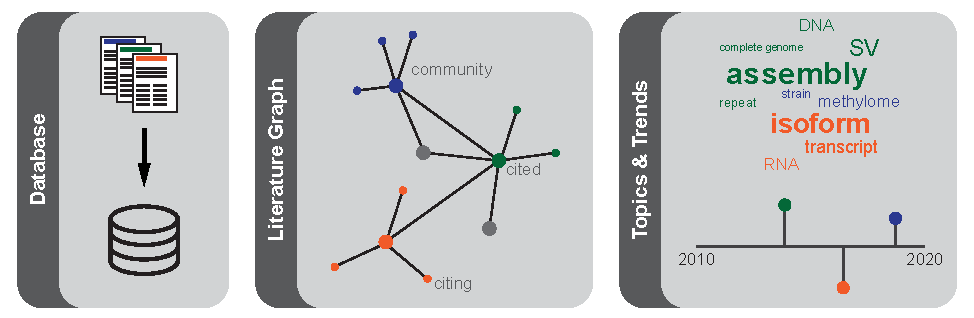
\includegraphics[width=1.0\textwidth]{figures/state_of_art/GA.pdf}
	\label{fig:state_of_art:ga}
\end{figure}

The chapter starts with a \textbf{background} in \ref{sec:state_of_art:background} followed by the setup and usage of a \textbf{literature database} containing scientific publication meta data in \ref{sec:state_of_art:database}. A big picture overview of \textbf{third generation sequencing} technologies in \ref{sec:state_of_art:third_generation}, is followed by a focus on \textbf{nanopore sequencing} in \ref{sec:state_of_art:nanopore}. Finally, most recent \textbf{throughput and accuracy} benchmarks on in-house data close the state-of-the-art evaluation.




\section{Background}
\label{sec:state_of_art:background}

% stretch a bit more the general usage, not only for the novel nanopore field

The number of studies published per year in scientific journals is exponentially growing (Fig. \ref{fig:state_of_art:paper_count}).
Including only records with a digital object identifier (DOI) tracked by CrossRef and Semantic Scholar, results in a conservative estimation of 100k journals and a total of 5M paper being published only in 2020.
While the targeted discovery of specific studies remains feasible by indexing in search engines, the extensive and continuous tracking of an entire field of research becomes increasingly difficult.
Especially for the fast evolving field of nanopore sequencing, a zoomed out perspective is equally valuable for the orientation of newcomers and adaptation to latest developments in experienced groups.
A data driven literature scan facilitates the clustering of results and identification of key publications in an unbiased way.

%Zoom out history \cite{Deamer2016}
% axis labels capital, explain journal >= 5years, align legends to y-axis

\begin{figure}[h]
	\centering
	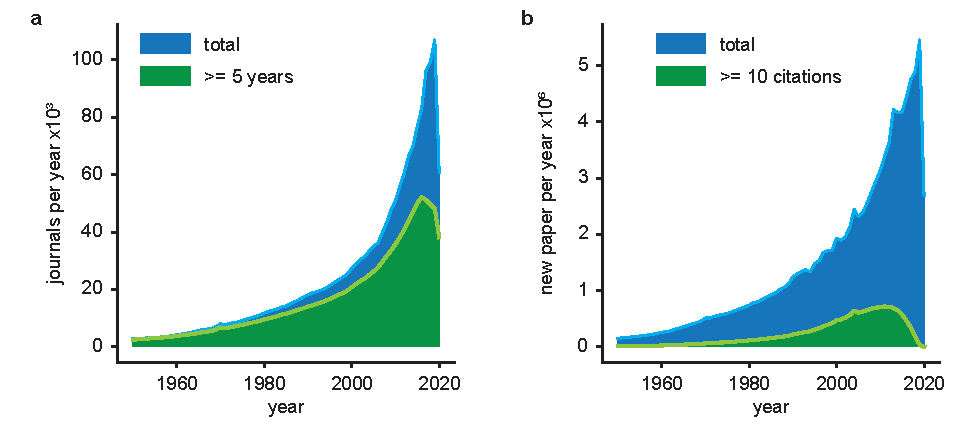
\includegraphics[width=1.0\textwidth]{figures/state_of_art/paper_count.pdf}
	\captionsetup{format=plain}
	\caption[Journals and publications per year]{Journals and new publications per year: \textbf{a}, Actively publishing scientific journals per year and journals with a publication history of at least five years. \textbf{b}, New publications per year and publications with at least 10 citations. (Semantic Scholar and CrossRef combined, only records with DOI)}
	\label{fig:state_of_art:paper_count}
\end{figure}

The following computer aided literature analysis is inspired by the Open Syllabus Galaxy\footnote{\url{https://galaxy.opensyllabus.org/}, accessed 01/2021} project.
Based on co-assignments of books in North American university courses, their literature graph of 160k books visualizes the linkage between research fields.
Applied to scientific journal publications, the success of the method is limited by the availability and quality of large scale meta data such as title, abstract and citations.
A number of platforms like Google Scholar, Web of Science, Dimensions or Microsoft Academic operate online literature databases, though without access to larger data chunks for systematic offline analysis.
Additional full text for advanced text mining is commonly only available through paid access from individual journals.




\section{Literature Database}
\label{sec:state_of_art:database}

For the purpose of tracing citations and clustering larger numbers of publications, we first setup a custom literature database.
The Semantic Scholar open research corpus (S2ORC) provides the largest available collection of scientific paper meta data and serves as starting point in this work \cite{Lo2020}.
Collected 07/2020, the data contains 77M papers linked by 333M citations.
Provided as compressed JSON files, the records are re-organized into a SQLite database with two main tables for records and citations.
Each record is uniquely identified by it's DOI and can additionally contain year, journal, title and abstract.
Citations are unique pairs of citing and cited DOI, referencing rows in the records table.
To further improve completeness of records and citations, we incrementally query the CrossRef REST API\footnote{\url{https://github.com/CrossRef/rest-api-doc}, accessed 01/2021} for novel entries, most recently in January 2021.
Citations are part of CrossRef but not provided through the API.
The CrossRef Open Citations Index (COCI) however, is regularly parsing and dumping citations and therefore integrated as well \cite{Peroni2020}.
Metrics of the final database used for this work are summarized in table \ref{tab:state_of_art:graph}. 
For comparison, the Dimensions\footnote{\url{https://www.dimensions.ai/}, accessed 01/2021} online platform lists 114M records and 1.3G citations.

\begin{table}[ht]
	\centering
	\caption[Literature Graph Metrics]{Literature database metrics}
	\label{tab:state_of_art:graph}
	\begin{tabular}{l|r}
		\hline
		citations (edges)           & 901 M 	\\
		paper (nodes)               & 116 M 	\\ \hline
		with title					& 115 M		\\
		with title \& abstract		&  57 M		\\ \hline
		connected nodes             &  68.4 M 	\\
		> 0 citations				&  56.6 M	\\
		> 5 citations				&  27.5 M	\\
		largest connected component &  67.9 M 	\\ \hline
	\end{tabular}
\end{table}

The network of publications and citations can also be interpreted as a literature graph with papers as nodes and citations as edges.
Only a fraction of 68M publications has either citing or cited edges.
The lack of citing (outgoing) edges indicates insufficient parsing of the papers reference sections, while the lack of cited (incoming) edges is likely a combination of technical limitations and unrecognized publications.
Striking though, is the presence of the largest connected component of 67.9M publications, where each paper can be reached via at least one citation edge.

A subset of publications originating from the S2ORC data set is annotated with a primary field of research from Microsoft Academic (MA). 
To get a first impression of the value of a literature graph, we first extracted all edges connecting papers with an annotated field of research.
Next, a hierarchical clustering of summarized citation counts per field is plotted as heatmap in Fig. \ref{fig:state_of_art:field_interactions}, and shows an intuitive grouping of natural- and social sciences.

\begin{figure}[h]
	\centering
	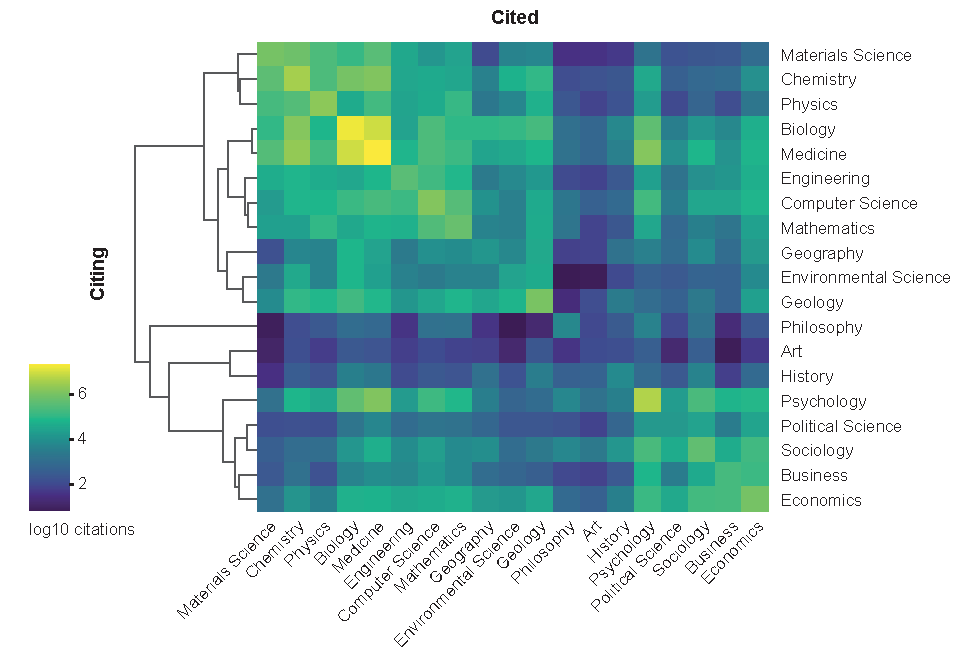
\includegraphics[width=1.0\textwidth]{figures/state_of_art/field_interactions.pdf}
	\captionsetup{format=plain}
	\caption[Scientific field interactions]{Citation edges summarized by field of research: Sum of citations (log10) between and within fields of research (Hierarchical clustering, method: centroid, distance: cosine).}
	\label{fig:state_of_art:field_interactions}
\end{figure}

A graph is a powerful data structure, for instance to detect local communities or compute distances between nodes, however, with a growing number of nodes and edges it becomes impossible to visualize.
For the purpose of visualization and clustering, a graph embedding, similar to the \textit{node2vec} algorithm used in the OpenSyllabus project is therefore needed \cite{Grover2016}.
A graph embedding is a fixed length vector representation of each node, with the aim to preserve local connectivity.

The vector representation is enabling distance based clustering methods such as KMeans and dimensional reduction by principal component analysis (PCA) and uniform manifold approximation (UMAP).
Additionally, while sub-sampling nodes of a graph would split connected components, sub-sampling from an embedded graph, based on e.g. citation counts or topic, preserves the overall structure and reduces required compute resources.

Embedding the scientific literature graph using \textit{node2vec} is due to run-times of multiple weeks on CPU and large memory requirements on GPU not feasible.
We use therefore the \textit{DeepWalk} \cite{Perozzi2014} algorithm with its GPU implementation in \textit{GraphVite} \cite{Zhu2019}.
In order to fit on a GPU-server with 4x NVIDIA 2080Ti (11 GB RAM), only edges connecting publications with at least 20 citations are considered.
The resulting sub-graph, in the following referred to as \textbf{core\_20} graph, contains 9M nodes encompassed by virtually a single connected component.

Embedding with default parameters yields feature vectors of length 128 for each publication.
Following the OpenSyllabus projects workflow, the high-level visualization in Fig. \ref{fig:state_of_art:umap_global} is generated by first reducing to 64 dimensions using PCA (85\% explained variance), followed by further reduction to two dimensions using a UMAP.
For a better overview, only publications with fields considered relevant for this work are shown.

\begin{figure}[h]
	\centering
	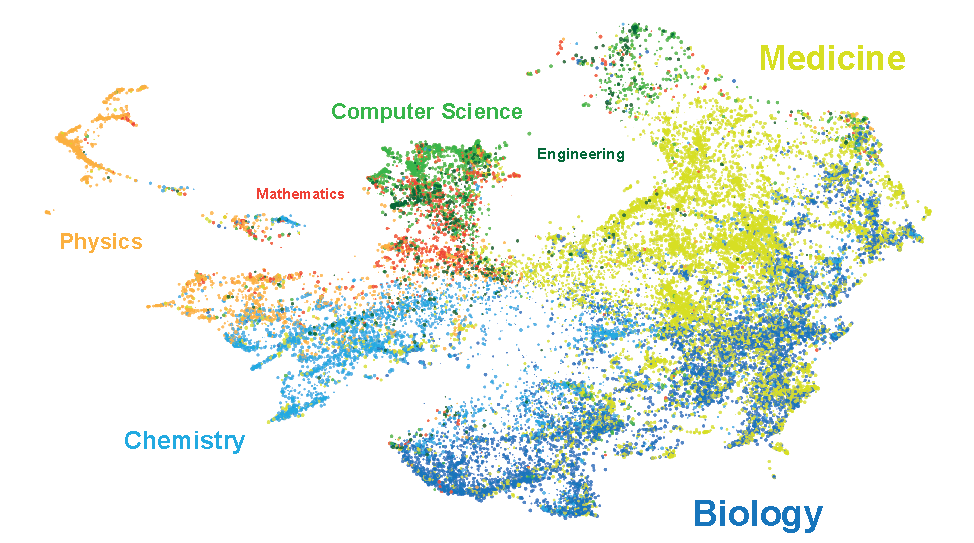
\includegraphics[width=1.0\textwidth]{figures/state_of_art/umap_global.pdf}
	\captionsetup{format=plain}
	\caption[Scientific literature graph]{Scientific publication graph embedding: UMAP visualization of \textit{DeepWalk} graph embedding colored by field of research. Publications from 1980 onward with at least 20 citations (n=9M embedded, n\_neighbors 75, min\_dist 0.01, metric correlation, n=50k random sample of relevant fields plotted).}
	\label{fig:state_of_art:umap_global}
\end{figure}

In summary, the gathered SQLite literature database supports a variety of fast queries for e.g. research fields, journals, year of publication or citations.
The graph embedding of highly cited publications is a proof of concept to visualize literature based on citations and provides an intuitive perspective on field interactions.
Due to automated parsing, lack of visibility but also novelty of a paper, a considerable part of the database can not be embedded.
To address this issue, a future version with weighted pseudo-citations based on text similarities is planned.




\section{Third Generation Sequencing}
\label{sec:state_of_art:third_generation}

Both, the \textit{Nanopype} pipeline in chapter \ref{cha:nanopype} and \textit{STRique} repeat detection in chapter \ref{cha:strique} are exclusively developed for nanopore sequencing data.
Nevertheless, from a review perspective, both long read platforms are of interest, in particular when portability or initial acquisition cost play a secondary role.
The identification of third generation sequencing related publications is implemented in three steps of seed, extend and connect.
First, publications with keywords in either title or abstract are marked as seed paper.
The second step extends clusters around seed papers by following their citation edges in the literature graph.
Lastly, additional edges derived from text similarities and random walks in the \textbf{core\_20} backbone graph reduce the sparsity of the third generation citation graph.

Title and abstract columns of the records table are indexed for full text search using the SQLite \textit{FTS5} extension. 
For PacBio SMRT sequencing, the respective query is 'pacbio OR single molecule real time sequencing', for ONT 'nanopore sequencing' is used.
\textit{FTS5} is case-insensitive and works based on tokens, 'sequencing' for instance, is stemmed to 'sequenc', requiring a post processing step to validate matches and reduce false positives.
The number of seed papers for PacBio is 2900, for ONT 2852 paper contain the words 'nanopore' and 'sequencing' in title or abstract.
The output is comparable to the online platform Dimensions, which lists 3147 publications for 'nanopore sequencing' (queried 01/2021).

The extension of paper clusters around keywords is achieved by iteratively adding publications with a minimum number of citations and with a strong binding to the cluster.
The binding is computed as the fraction of in- or outgoing edges reaching nodes in the current cluster.
The seed extension is evaluated for different parameter combinations, with five citations and a minimum binding of 0.2 resulting in the largest stable cluster (Fig. \ref{fig:state_of_art:cluster_convergence}).
The PacBio and Nanopore cluster grow to similar sizes of 4392 and 4689 publications respectively and form the third generation sequencing cluster. 
The number of nodes reached by both extensions though, is with 308 unexpectedly low.

\begin{figure}[h]
	\centering
	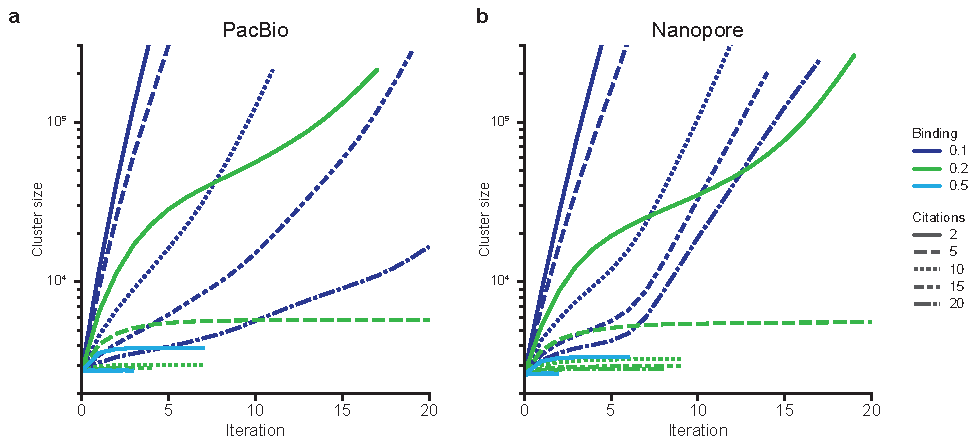
\includegraphics[width=1.0\textwidth]{figures/state_of_art/cluster_convergence.pdf}
	\captionsetup{format=plain}
	\caption[Keyword Seed and Extend Convergence]{Cluster size convergence of keyword seed and extend strategy for PacBio query (\textbf{a}) and ONT query (\textbf{b}). The iteration is stopped on convergence, after 20 steps or on exceeding a threshold of 50k publications.}
	\label{fig:state_of_art:cluster_convergence}
\end{figure}

To further link isolated connected components and for additional preservation of the global graph structure, we complement the extracted third generation sub-graph by random walks in the \textbf{core\_20} backbone graph.
Each walk starts at a sub-graph node which is also contained in the \textbf{core\_20} graph and follows citation edges within the \textbf{core\_20} backbone, until another shared node is found, or a maximum length is reached.
Edges of random walks are only used for embedding, the additional nodes are ignored in the subsequent content analysis.
Of the initial 8.7k third generation sequencing sub-graph nodes, only 7.6k have citing or cited edges suitable for embedding.
In order to also integrate publications without citations, we add additional weighted edges based on text similarities between documents.
Specifically, a MinHash LSH Forest is used to perform top-k queries based on approximated Jaccard similarities \cite{Bawa2005}.
The LSH Forest is build of hashed titles and abstracts of all publications in the random walk expanded third generation sequencing graph.
For each publication, edges to the top 500 most similar documents in the set are stored as candidates, with the approximated Jaccard similarity as weight.
Of all candidate edges, the top 20\% edges between highly similar documents are added to the third generation sequencing graph.
For the embedding, the graph is treated as un-directed and weighted, with a constant weight of 1.0 assigned to all citation edges.
Applying the same \textit{DeepWalk} configuration and dimensionality reduction as above results in the third generation sequencing graph embedding shown in Fig. \ref{fig:state_of_art:umap_lr}.

\begin{figure}[h]
	\centering
	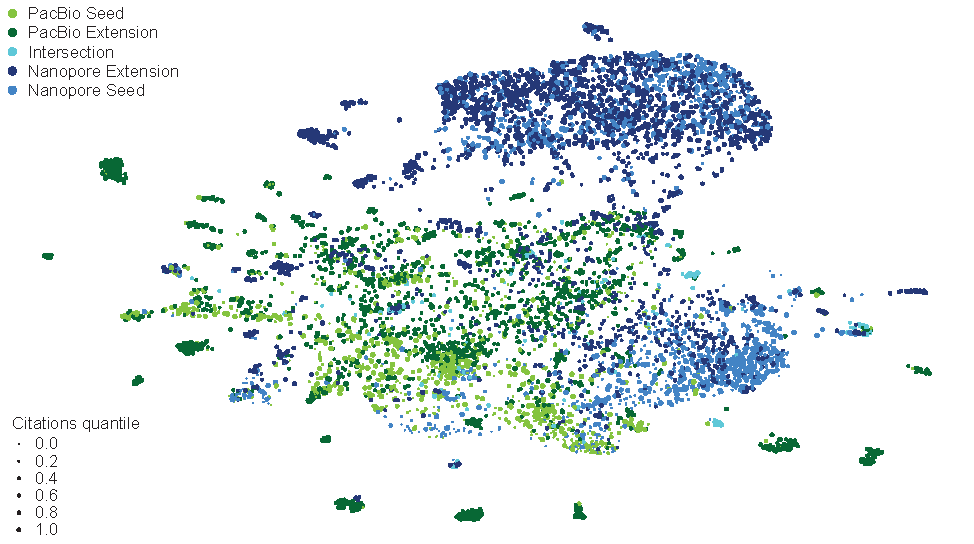
\includegraphics[width=1.0\textwidth]{figures/state_of_art/umap_lr.pdf}
	\captionsetup{format=plain}
	\caption[Third generation sequencing cluster]{Third generation sequencing cluster: The UMAP projection shows the \textit{DeepWalk} graph embedding with points scaled by number of citations. Colors indicate technology and seed/extend source.}
	\label{fig:state_of_art:umap_lr}
\end{figure}

The third generation literature graph embedding reveals a largely separated field of publications relying on either Pacific Biosciences or Oxford Nanopore Technologies.
Aside from small outlier groups, a broad PacBio field is accompanied by three distinct accumulations of nanopore related work.
The embedding of the third generation sequencing sub-graph is clustered after discarding nodes added by the random walk expansion.
Using the KMeans algorithm, an optimal number of clusters is found with 24 based on the distortion score.
A subsequent hierarchical clustering of cluster centers results in a distance based sorting (Fig. \ref{fig:state_of_art:cluster_sizes} a).
The ratio of seed to extension papers per technology and cluster confirms the previously noted separation of PacBio and ONT (Fig. \ref{fig:state_of_art:cluster_sizes} b).
Aside from small clusters of virtually only extension publications (ID 0, 6-7, 17-19), two major groups, of which one (ID 20-23) contains only nanopore seeds and extensions, become visible.
Remarkable is, that clusters with on average older publications tend to have a higher proportion of extensions, indicating, that the extension of the novel third generation field is primarily directed towards older publications, defining the broader field of application.
In return, the clusters with the highest mean citation counts are 12, 15, 22 and 23, each with high seed to extend ratios.
These clusters are in the following identified as core-assembly, MinION usage, solid state pore development and analysis of pore translocating polymers.

\begin{figure}[h]
	\centering
	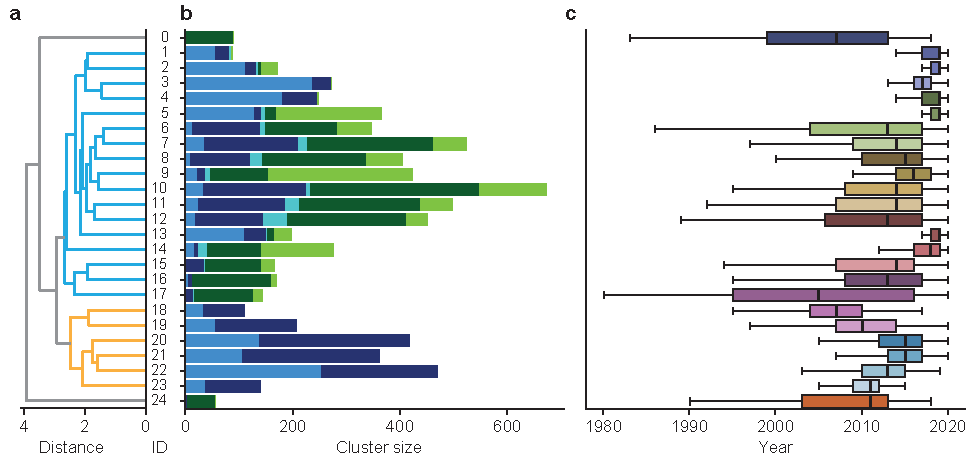
\includegraphics[width=1.0\textwidth]{figures/state_of_art/cluster_sizes.pdf}
	\captionsetup{format=plain}
	\caption[Long-Read Application Cluster]{Cluster of long-read applications: \textbf{a}, Hierarchical clustering of cluster centers assigns cluster IDs based on inter-cluster distance. \textbf{b}, Cluster size, seed to extend and technology composition are shown as stacked bar plots. \textbf{c}, Distributions of publication years per cluster with data as boxplots (centerline, median; box limits, first and third quartiles; whiskers, 1.5x interquartile range).}
	\label{fig:state_of_art:cluster_sizes}
\end{figure}

Word clouds provide an intuitive way for high-level content analysis of each cluster.
First, titles and abstracts are split into word tokens and further reduced to their stem using the Porter Stemming Algorithm.
Descriptive tokens are extracted using a term-frequency inverse-document-frequency (TF-IDF) embedding.
After filtering out tokens occurring in less than 10 documents or more than 20\% of the corpus, each token in each document is assigned a score based on how frequent it is mentioned in the document (for titles and abstracts commonly once) as opposed to how frequent it is found in the corpus.
The result is a word embedding matrix of 8k third generation sequencing publications times 4.6k descriptive word tokens.
After averaging TF-IDF scores per cluster, each clusters top 200 highest scoring tokens are illustrated as word clouds, of which three examples are shown in Fig. \ref{fig:state_of_art:wcs_minion}.

\begin{figure}[h]
	\centering
	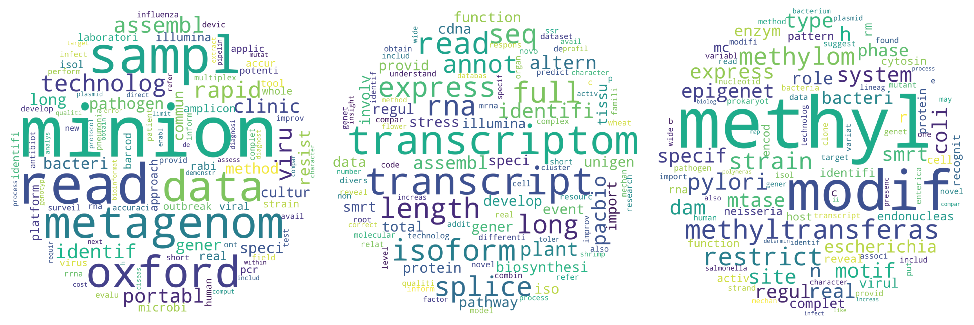
\includegraphics[width=1.0\textwidth]{figures/state_of_art/wcs_minion.pdf}
	\captionsetup{format=plain}
	\caption[Nanopore Sequencing Word Clouds]{Nanopore sequencing word clouds of cluster 1, 15 and 16 reveal a virus identification, a composite cluster around the usage of the MinION and an algorithmic cluster around assembling, error correction and alignments.}
	\label{fig:state_of_art:wcs_minion}
\end{figure}

Not all word clouds can be translated into meaningful cluster labels.
Especially cluster with few publications or a low seed to extension ratio are difficult to characterize.
Nonetheless, for most clusters a high-level label is found and annotated into the graph embedding (Fig. \ref{fig:state_of_art:umap_cluster}).
Surprisingly, while referring to nanopore sequencing, the isolated clusters (ID 20-23) have no direct reference to Oxford Nanopore Technologies, but cover the development of novel protein and graphen based nanopores, translocating polymer and signal analysis.
Beyond that, the token 'assembl' (words: assembly, assemble, assembling etc.) is one of the most prominent, and with different scalings found in almost all clusters.

\begin{figure}[h]
	\centering
	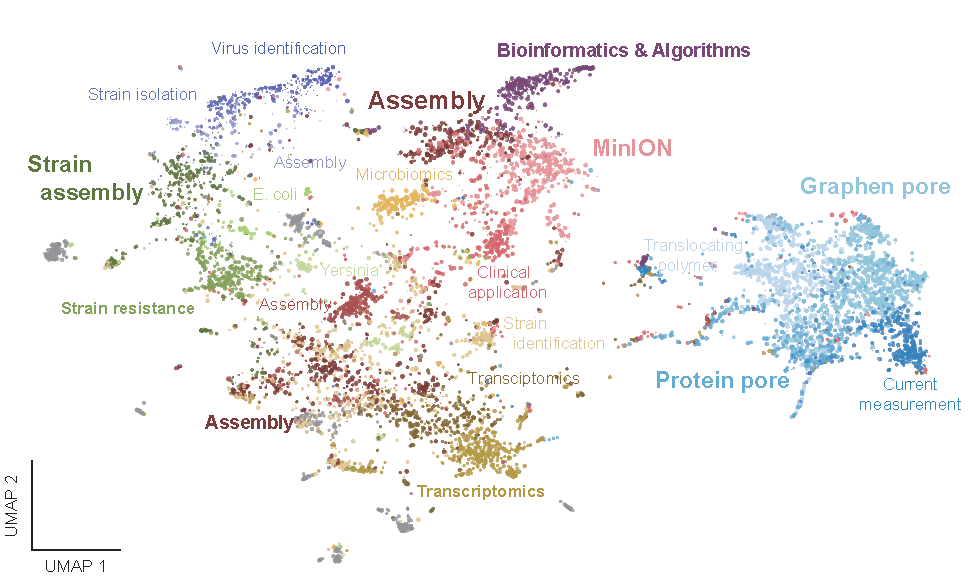
\includegraphics[width=1.0\textwidth]{figures/state_of_art/umap_cluster.pdf}
	\captionsetup{format=plain}
	\caption[Third generation sequencing applications]{Third generation sequencing applications: The UMAP projection shows the \textit{DeepWalk} graph embedding with points scaled by number of citations (1 for content linked publications). Colors indicate cluster with labels derived of most descriptive word tokens.}
	\label{fig:state_of_art:umap_cluster}
\end{figure}

The following section aims to provide a brief insight into major application fields for long-read sequencing technologies, while in particular highlighting the contribution of nanopore sequencing.
Key publications are determined as highly cited paper per year, in comparison to their respective cluster community.
In clusters with only few seed publications, these are primarily mentioned to emphasize the role of the technology within the field.

\textbf{Limitations:} 
While so far providing a data-driven high-level overview of the third generation sequencing field, the following section is referring to individual publications based on citation counts.
By citing what is already highly recognized, a bias against very new or comparably small application fields is anticipated.
An example are the already visible tokens 'sar' and 'cov' in the virus identification cluster.
Contributing to an emerging application field of assembling variants and detecting mutations of the SARS-CoV-2 virus, associated key publications based on citation counts are still impossible to obtain using our database.




\section{Nanopore Sequencing Applications}
\label{sec:state_of_art:nanopore}

Publications of the composite 'MinION' cluster (ID 15) receive, with an average of 28, the most citations.
Followed by 18 for the 'Assembly' cluster (ID 12) and 16 for 'Bioinformatics \& Algorithms' (ID 16), these clusters form the most recognized section of the third generation sequencing field.
None of the other clusters is reaching more than 11 citations on average.
Based on a first inspection, these highly cited clusters contribute primarily methods and proof of concept studies, while the surrounding clusters define the broader field of application with in detail very specific studies.
Major application fields are identified as:

\begin{packed_enum}
	\item Bioinformatics
	\item Assembly
	\item Structural variant detection
	\item Bacterial and viral strain analysis
	\item Metagenomics and microbiomics
	\item Isoform detection
\end{packed_enum}

For the 'MinION' cluster in general and otherwise where appropriate, publications are mentioned in the context of their primary usage, regardless of their cluster assignment.
An interesting example is the interplay of 'Bioinformatics \& Algorithms' and the 'Assembly' arm of the bacterial strain analysis field (Fig. \ref{fig:state_of_art:cluster_sizes} ID 16 and 3, Fig. \ref{fig:state_of_art:umap_cluster} light purple and dark red).
While a variety of tools and pipelines for \textit{de-novo} genome assembly have been published, the most prominent \textit{Canu} \cite{Koren2017} is assigned to cluster ID 3, pulled towards its application to bacterial and viral strains.
A central cluster with respect to the UMAP projection (Fig. \ref{fig:state_of_art:umap_cluster}, ID 14) covers clinical applications. Yet individual publications rely on methods of the surrounding clusters, for example detection of disease associated structural variations or analysis of antibiotic-resistant strains.
So far not visible as independent cluster, but of particular interest for this work, is the detection of epigenetic base modifications using nanopore sequencing.
An according section with current methods and proof of concept studies is therefore appended.




\subsection{Bioinformatics}
\label{subsec:state_of_art:bioinf}

Significantly longer reads, in combination with higher error rates compared to NGS technologies, require adaptation of existing and development of novel bioinformatics software.
Among the earliest publications are tools providing \textbf{simulations} of SMRT sequencing data \cite{Ono2013, Stoecker2016}.
Virtually unlimited amounts of artificial long reads with characteristic length distributions and error profiles facilitate early development and testing of downstream applications, independent of the real data throughput at the time.
Similar tools exist for nanopore signal and sequence data, but are not visible by their citations.
With existing data and experience from SMRT sequencing, we hypothesize, that the nanopore versions are primarily for the development and debugging of for instance streaming algorithms and become less important with more real data being publicly available.
%Simulation (SMRT):
%PBSIM: PacBio reads simulator—toward accurate genome assembly \cite{Ono2013}
%SimLoRD: Simulation of Long Read Data \cite{Stoecker2016}

Despite ongoing improvements, the error rate of third generation sequencing technologies requires constant quality control. Particularly for nanopore sequencing, a number of \textbf{visualization} packages have been developed.
Initially receiving a lot of attention, none of \textit{Poretools} \cite{Loman2014},
\textit{PoRe} \cite{Watson2014} or \textit{NanoOK} \cite{Leggett2016} is actively maintained and would be able to handle the most recent ONT file formats.
Functional and under active development is \textit{NanoPack} \cite{DeCoster2018}, supporting both, SMRT and nanopore data.

Translating the primary signal into sequences during \textbf{basecalling} is a crucial processing step for third generation sequencing reads.
High-fidelity (HiFi) SMRT reads and advancing algorithms for nanopore basecalling render initial read-level error correction methods obsolete \cite{Koren2012, Hackl2014, Goodwin2015}.
For nanopore reads, the single read accuracy has increased from \textasciitilde85\% using the cloud-based \textit{Metrichor} over \textasciitilde87\% in \textit{albacore} to 95\% in the most recent recurrent neural network basecaller \textit{guppy}.
Clearly headed by the manufacturers, a couple of community methods have been proposed, namely 
\textit{DeepNano} \cite{Boza2017} \textit{Nanocall} \cite{David2017} and \textit{Chiron} \cite{Teng2018}.
Although free and open-source, these are not competitive in terms of accuracy and run time.
The performance of neural network basecalling tools for ONT data has recently been reviewed \cite{Wick2019}.
Yet, the ongoing improvement of production grade, and promising experimental platforms such as \textit{bonito}\footnote{\url{https://github.com/nanoporetech/bonito}}, require constant quality assessment on patch to patch level.

Shared by most downstream applications is the \textbf{alignment} of reads against a reference genome.
The first recognized long read aligner is \textit{BLASR} \cite{Chaisson2012}, maintained by PacBio and for SMRT reads only.
Published in 2016, \textit{minimap} \cite{Li2016} and \textit{GraphMap} \cite{Sovic2016} are both developed for long, noisy read alignments.
While \textit{minimap} computes very fast approximate mappings, \textit{GraphMap} is very sensitive, but requires, due to its reference index structure, considerably more memory.
Actively improved and maintained in version two, \textit{minimap2} \cite{Li2018} and \textit{GraphMap2} \cite{Maric2019} additionally support spliced alignments of transcript reads.
The fast and memory efficient algorithm of \textit{minimap2} makes it to one of the most used aligners in the field.
An aligner, especially developed for the mapping of structural variations is \textit{NGMLR} \cite{Sedlazeck2018}.
Splitting of reads into fragments of few kilobases, and subsequent individual alignment using a convex gap cost model, improves the accurate detection of breakpoints.
Using parameter presets, \textit{minimap2}, \textit{GraphMap2} and \textit{NGMLR} are capable of mapping both, SMRT and nanopore reads.




\subsection{Assembly}
\label{subsec:state_of_art:assembly}

\textit{De-novo} assembling of previously unknown and improving the quality of existing draft genomes is a primary application of long read sequencing.
Assembling greatly benefits from increased throughput per flow cell, read-lengths and single-read accuracy, replacing next- by third-generation technologies as current gold standard.
Both, PacBio and ONT enable state-of-the-art genome assemblies, especially for viral and bacterial genomes.
The choice of a suitable platform therefore also depends on already available data, portability and instrument acquisition cost.
Limited by throughput and accuracy, initial SMRT assemblies focused on the scaffolding and completion of existing bacterial draft genomes \cite{English2012, Boetzer2014}.
Hybrid approaches combine next- and third-generation sequencing data, and thus integrate the accuracy of short reads with the continuity of noisy long-reads \cite{Bashir2012, Antipov2016}.
%Mind the Gap: Upgrading Genomes with Pacific Biosciences RS Long-Read Sequencing Technology \cite{English2012}
%SSPACE-LongRead: scaffolding bacterial draft genomes using long read sequence information \cite{Boetzer2014}
%A hybrid approach for the automated finishing of bacterial genomes \cite{Bashir2012}
%hybridSPAdes: an algorithm for hybrid assembly of short and long reads \cite{Antipov2016}
First third-generation-only assemblies include a finished fungal genome (\textit{Verticillium dahliae}, 35Mb) \cite{Faino2015} based on SMRT reads and optical mappings and a nanopore-only assembly of \textit{Escherichia coli} (4.6Mb) \cite{Loman2015}.
%Single-Molecule Real-Time Sequencing Combined with Optical Mapping Yields Completely Finished Fungal Genome \cite{Faino2015}
%A complete bacterial genome assembled de novo using only nanopore sequencing data \cite{Loman2015}
More recently, studies report the successful assembly of \textasciitilde80\% of the hexaploid wheat genome (\textit{Triticum aestivum}, 17Gb) with NG50s of 88kb and 480kb \cite{Clavijo2017, Zimin2017} and an improved maize reference (\textit{Zea mays }, 2.1 Gb, NG50 1.2Mb) \cite{Jiao2017}, each using SMRT sequencing in combination with optical mapping.
%An improved assembly and annotation of the allohexaploid wheat genome identifies complete families of agronomic genes and provides genomic evidence for chromosomal translocations \cite{Clavijo2017}
%Improved maize reference genome with single-molecule technologies \cite{Jiao2017}
%Hybrid assembly of the large and highly repetitive genome of Aegilops tauschii, a progenitor of bread wheat, with the MaSuRCA mega-reads algorithm \cite{Zimin2017}
Further examples of improved genome sequences are tea (\textit{Camellia sinensis var. sinensis}, 3.1Gb, NG50 1.4Mb) \cite{Wei2018}  and apple (\textit{Malus x domestica}, \textasciitilde700Mb, NG50 7.0Mb) \cite{Zhang2019}, with the latter using a combination of optical mapping and Hi-C (Chromosome conformation capture) data for scaffolding.
%Draft genome sequence of Camellia sinensis var. sinensis provides insights into the evolution of the tea genome and tea quality \cite{Wei2018}
%A high-quality apple genome assembly reveals the association of a retrotransposon and red fruit colour \cite{Zhang2019}
In summary current state-of-the-art chromosome-scale assemblies of large, potentially di- or polyploid genomes can be build solely based on SMRT or nanopore reads in combination with optical mapping and/or Hi-C data for scaffolding \cite{Belser2018}.
%Chromosome-scale assemblies of plant genomes using nanopore long reads and optical maps \cite{Belser2018}

A number of standalone tools and pipelines for genome assembly have been published.
% strain assembly, 2400 citations
% Canu: scalable and accurate long-read assembly via adaptive k-mer weighting and repeat separation \cite{Koren2017}
% strain resistance, in long read mode using racon and miniasm \cite{Li2016}, 1400 citations
% Unicycler: Resolving bacterial genome assemblies from short and long sequencing reads \cite{Wick2017}
Based on their citations, \textit{Canu} \cite{Koren2017} and \textit{Unicycler} \cite{Wick2017a} are the most used assembly pipelines. Both are not assigned to the core-assembly cluster (ID 12, 13), but are part of the strain-assembly and strain-resistance cluster respectively, highlighting their importance for a large user group.
% FALCON, 540 citations
% Phased diploid genome assembly with single-molecule real-time sequencing \cite{Chin2016}
Developed exclusively for SMRT sequencing is \textit{FALCON} \cite{Chin2016}, with the additional function of phasing diploid genomes.
% minion cluster 622 citations
% Racon: Fast and accurate de novo genome assembly from long uncorrected reads \cite{Vaser2017}
\textit{Racon} \cite{Vaser2017} and \textit{miniasm} \cite{Li2016} are lightweight standalone assembly tools, both assigned to the 'MinION' composite cluster. 
Together they are forming the computational backend of \textit{Unicycler} when processing long-reads and \textit{Racon} is performing the initial consensus assembly of transcript reads in the ONT isoform detection pipeline \textit{Pinfish}\footnote{\url{https://github.com/nanoporetech/pinfish}, accessed 02/2021}.
% minion cluster
%Nanopore sequencing and the Shasta toolkit enable efficient de novo assembly of eleven human genomes \cite{Shafin2020}
Two important standalone assemblers published in 2020 are \textit{Flye} \cite{Kolmogorov2019} and \textit{Wtdbg2} \cite{Ruan2020}, both missed by the data driven state-of-the-art analysis so far.
Both abstracts do not contain a direct reference to either one of the long-read technologies and despite having already high citation counts, both are not reached by the extension strategy.
This example points to two shortcomings of the proposed literature mining strategy: First, it is only sensitive to topics (tokens) present in title and abstract.
Second, its success and coverage are decisively impacted by the seed-extension strategy.
Nonetheless, if specifically interested in assembling, the token 'assembl' would have picked up both examples as seed publications.

Similar to the continuous improvement of basecalling algorithms, the assembly field is advancing at a fast paste.
Published in 2018, Jain et al. report the linear assembly of the centromere on the human Y chromosome and later the assembly of a human genome using only nanopore long-reads \cite{Jain2018, Jain2018b}.
%Linear assembly of a human centromere on the Y chromosome \cite{Jain2018}
%Nanopore sequencing and assembly of a human genome with ultra-long reads \cite{Jain2018b}
Only two years after publication, the reported NG50 of 6.4Mb based on \textit{Metrichor} basecalling and \textit{Canu} assembly is clearly outperformed by more recent workflows.
An in-house benchmark of \textit{Flye} on a human data set with 30X coverage and 20kb N50 read length lead to a draft genome assembly with 25Mb NG50, further outperformed by the developer benchmark, reporting up to 40Mb NG50 using comparable coverage\footnote{\url{https://github.com/fenderglass/Flye}, accessed 02/2021}.




\subsection{Structural Variant and Haplotype Resolution}
\label{subsec:state_of_art:sv}

Structural variations (SVs) describe differences, for instance deletions, insertions, or translocations, between individual genomes and a reference sequence.
On individual base level, single-nucleotide polymorphisms (SNP) are substitutions of single bases in the genome, observable in a fraction of a population.
Both variation types are detectable by NGS technologies, advantages of long-read sequencing are the accurate detection of large variants and the long-distance haplotype resolution based on SNPs.
With no dedicated cluster for structural variant detection, respective tools got assigned to the bioinformatic cluster (ID 16), while applications are mostly found within the clinical application cluster (ID 14).
Currently available SV detection tools include \textit{NanoSV} \cite{Stancu2017}, \textit{Sniffles} \cite{Sedlazeck2018} and \textit{SVIM} \cite{Heller2019}.
With sequence alignments as inputs, these are commonly applicable to SMRT and nanopore reads.
The performance is, however, influenced by the preceding alignment, finding the combination of \textit{minimap2} and \textit{Sniffles} the currently most sensitive and fastest option \cite{Coster2019}.
% NanoSV
%Mapping and phasing of structural variation in patient genomes using nanopore sequencing \cite{Stancu2017}
%Missing NRMLR/Sniffles \cite{Sedlazeck2018}
%SVIM: structural variant identification using mapped long reads \cite{Heller2019}
% sniffles vs svim evaluation on minimap2 and NGMLR alignment
%Structural variants identified by Oxford Nanopore PromethION sequencing of the human genome \cite{Coster2019}

The analysis of human leukocyte antigen (HLA) variants is a major clinical application relying on both, NGS and third-generation sequencing.
The polymorphic HLA genes are essential for the human immune system. 
Before organ transplantation, their characterization is essential to minimize the chance of rejection by the receiving patient.
In addition to high-throughput NGS methods, both SMRT and nanopore sequencing are applied to detect HLA variants \cite{Cereb2015, Ammar2015}, leading to characterizations of novel and confirmation of know alleles \cite{Albrecht2017}.
%
% single minion flow-cell, R7 pore, limited by low throughput
% Long read nanopore sequencing for detection of HLA and CYP2D6 variants and haplotypes \cite{Ammar2015}
% HLA molecular testing service
% Advances in DNA sequencing technologies for high resolution HLA typing \cite{Cereb2015}
% Dual redundant sequencing strategy: Full-length gene characterisation of 1056 novel and confirmatory HLA alleles \cite{Albrecht2017}
%
% SMRT enrichment
% delineating the breakpoint junctions of low copy repeat (LCR)-associated complex structural rearrangements on chr17p11.2 in patients diagnosed with Potocki–Lupski syndrome (PTLS; MIM#610883). 
% PacBio-LITS: a large-insert targeted sequencing method for characterization of human disease-associated chromosomal structural variations \cite{Wang2015}
% Nanopore sequencing detects structural variants in cancer \cite{Norris2016}
% Profiling of Short-Tandem-Repeat Disease Alleles in 12,632 Human Whole Genomes \cite{Tang2017}
%
Furthermore, long-read sequencing is used to characterize disease-associated structural variations, for instance segmental duplications in patients with Potocki–Lupski syndrome (PTLS) \cite{Wang2015} or deletions causing tumor suppressor gene inactivation in pancreatic cancer \cite{Norris2016}.
Nonetheless, NGS still plays a major role, especially in the analysis of large patient cohorts, where available library preparation input material and sequencing cost have to be taken into account \cite{Tang2017}.




\subsection{Bacterial \& Viral Strain Analysis}
\label{subsec:state_of_art:strain}

The identification and analysis of viral and bacterial strains is, in terms of publication counts, the largest application field for long-read sequencing.
Significantly smaller genomes compared to mammals and plants facilitate the early adaptation of third-generation technologies by compensating the initial error rates with high sequencing coverage.
In stationary operation, the PacBio Sequel II and the ONT MinION appear to be equally well suited platforms.
However, based on citation counts, publications relying on the real-time and mobility aspect of the MinION stick out in the following.
In contrast to the massively parallel SMRT sequencing, individual reads from a nanopore sequencer can be analyzed directly after passing through the pore.
Proof of concept studies have demonstrated mobile nanopore sequencing in challenging environments on the International Space Station \cite{Castro-Wallace2017} and in the Antarctic \cite{Johnson2017}.
This section is subdivided into the mobile identification of viral strains (Cluster ID 1), analysis of bacterial antibiotic resistance (ID 5, 6) and metagenomic identification of bacterial and viral pathogens (ID 15).

%Nanopore DNA Sequencing and Genome Assembly on the International Space Station \cite{Castro-Wallace2017}
%Real-Time DNA Sequencing in the Antarctic Dry Valleys Using the Oxford Nanopore Sequencer \cite{Johnson2017}

% mobile virus
ebola, zika, lassa fever
Real-time, portable genome sequencing for Ebola surveillance \cite{Quick2016}
Mobile real-time surveillance of Zika virus in Brazil \cite{Faria2016}
Metagenomic sequencing at the epicenter of the Nigeria 2018 Lassa fever outbreak \cite{Kafetzopoulou2019}
Direct RNA nanopore sequencing of full-length coronavirus genomes provides novel insights into structural variants and enables modification analysis \cite{Viehweger2019}

% strain resistance
\textit{"Preventing, reducing, and controlling the emergence of antimicrobial-resistant organisms is a major public health challenge requiring the participation of the entire medical community and public health agencies."} \cite{Septimus2011}
Diverse antibiotic resistance genes in dairy cow manure \cite{Wichmann2014}
MinION nanopore sequencing identifies the position and structure of a bacterial antibiotic resistance island \cite{Ashton2015}
Rapid antibiotic-resistance predictions from genome sequence data for Staphylococcus aureus and Mycobacterium tuberculosis \cite{Bradley2015}
Streaming algorithms for identification of pathogens and antibiotic resistance potential from real-time MinION(TM) sequencing \cite{Cao2016}
Rapid Nanopore Sequencing of Plasmids and Resistance Gene Detection in Clinical Isolates \cite{Lemon2017}
Rapid inference of antibiotic resistance and susceptibility by genomic neighbour typing \cite{Brinda2020}

% pathogen
Rapid metagenomic identification of viral pathogens in clinical samples by real-time nanopore sequencing analysis \cite{Greninger2015}
Same-Day Diagnostic and Surveillance Data for Tuberculosis via Whole-Genome Sequencing of Direct Respiratory Samples \cite{Votintseva2017}
Nanopore metagenomics enables rapid clinical diagnosis of bacterial lower respiratory infection \cite{Charalampous2019}
Identification of bacterial pathogens and antimicrobial resistance directly from clinical urines by nanopore-based metagenomic sequencing \cite{Schmidt2017}

Rapid draft sequencing and real-time nanopore sequencing in a hospital outbreak of Salmonella \cite{Quick2015}
Rapid Pathogen Identification in Bacterial Pneumonia Using Real-Time Metagenomics \cite{Pendleton2017}
Completing bacterial genome assemblies with multiplex MinION sequencing \cite{Wick2017}




\subsection{Microbiomics}
\label{subsec:state_of_art:metagenomics}

Microbial phylogenetic profiling with the Pacific Biosciences sequencing platform \cite{Fichot2013}
Reducing assembly complexity of microbial genomes with single-molecule sequencing \cite{Koren2013}
Complete, closed bacterial genomes from microbiomes using nanopore sequencing \cite{Moss2020}

16s
Improved performance of the PacBio SMRT technology for 16S rDNA sequencing \cite{Mosher2014}
Sequencing 16S rRNA gene fragments using the PacBio SMRT DNA sequencing system \cite{Schloss2016}
Evaluation of PacBio sequencing for full-length bacterial 16S rRNA gene classification \cite{Wagner2016}
Species-level resolution of 16S rRNA gene amplicons sequenced through the MinION portable nanopore sequencer \cite{Benitez-Paez2016}




\subsection{Isoform Detection}
\label{subsec:state_of_art:isoform}

PacBio 4M reads per smart cell
Nanopore 5-10M for cDNA kit, 1M direct RNA kit

Both third-generation platform support the sequencing of full-length transcripts after conversion to cDNA. 
In addition are the nanopore devices by ONT capable of directly sequencing RNA, enabling the analysis of preserved RNA modifications.

Comprehensive comparison of Pacific Biosciences and Oxford Nanopore Technologies and their applications to transcriptome analysis \cite{Weirather2017}
A comprehensive examination of Nanopore native RNA sequencing for characterization of complex transcriptomes \cite{Soneson2019}

Characterization of Novel Transcripts in Pseudorabies Virus \cite{Tombacz2015}
Unveiling the complexity of the maize transcriptome by single-molecule long-read sequencing \cite{Wang2016}
A comprehensive approach to expression of L1 loci \cite{Deininger2017}
Characterization of the Dynamic Transcriptome of a Herpesvirus with Long-read Single Molecule Real-Time Sequencing \cite{Tombacz2017}
PacBio full-length cDNA sequencing integrated with RNA-seq reads drastically improves the discovery of splicing transcripts in rice \cite{Zhang2019a}
Full-length transcript characterization of SF3B1 mutation in chronic lymphocytic leukemia reveals downregulation of retained introns \cite{Tang2020}

Nanopore native RNA sequencing of a human poly(A) transcriptome \cite{Workman2019}

Potential but so far few publications
Accurate detection of m6A RNA modifications in native RNA sequences \cite{Liu2019}
Nanopore direct RNA sequencing maps the complexity of Arabidopsis mRNA processing and m6A modification \cite{Parker2020}

nanopore accuracy improvement in mid 2020




\subsection{Base Modification Detection}
\label{subsec:state_of_art:basemod}

Single-molecule real-time sequencing is sensitive for a number of base modifications, in particular N6-methyladenine (6mA) \cite{Flusberg2010}.
Modifications impact the kinetics of the polymerase while synthesizing the complementary strand, leading to characteristic pulse duration changes.
The sensitivity of SMRT sequencing for different modifications varies, the recommended coverage is ranging from 25X for 6mA to 250X for 5-methylcytosine (5mC) and 5-hydroxymethylcytosine (5hmC)\footnote{\url{https://www.pacb.com/wp-content/uploads/2015/09/WP_Detecting_DNA_Base_Modifications_Using_SMRT_Sequencing.pdf}, accessed 01/2021}.
With a focus on mammalian genomes and a primary interest in 5mC, such high coverage is, aside from sequencing costs, also not allowing for any single read analysis.
The sensitivity of nanopores to detect chemical base modifications, in particular 5mC and 5hmC, has already been reported in advance to the release of the ONT sequencing platform \cite{Laszlo2013, Schreiber2013}.
Modified bases cause a characteristic level change in the ionic current signal, which can be detected by downstream analysis software.
Both third-generation technologies can at individual-read and -base level only report a modification probability, leading to overall lower accuracy and missing values compared to whole genome bisulfite sequencing.
%Detection and mapping of 5-methylcytosine and 5-hydroxymethylcytosine with nanopore {MspA} \cite{Laszlo2013}
%Error rates for nanopore discrimination among cytosine, methylcytosine, and hydroxymethylcytosine along individual DNA strands \cite{Schreiber2013}

\textit{Nanopolish} \cite{Simpson2017} and \textit{SignalAlign} \cite{Rand2017} are the first tools detecting base modifications based on reads from the ONT MinION platform.
Developed for the R7 pore generation, \textit{Nanopolish} is reporting 5mC, \textit{SignalAlign} 6mA, 5mC and 5hmC.
However, only \textit{Nanopolish} is maintained, supporting the R9 pore and current raw signal file formats.
More recently, neural network based approaches in ONT \textit{Megalodon}\footnote{\url{https://github.com/nanoporetech/megalodon}}, \textit{DeepMod} \cite{Liu2019a} and \textit{DeepSignal} \cite{Ni2018} show promising accuracy improvements reviewed in \cite{Yuen2020}.
%Systematic benchmarking of tools for CpG methylation detection from Nanopore sequencing \cite{Yuen2020}
Yet, broad usability is hampered by non-standard output formats, lack of maintenance and complex software dependencies such as the ONT \textit{tombo}\footnote{\url{https://github.com/nanoporetech/tombo}} signal alignment and the \textit{tensorflow} environment.

Nanopore sequencing in epigenetics appears to be in a proof of concept and development state, with no demarcated publication cluster visible at the moment.
An example of its successful application is the rapid classification of brain tumors using nanopore sequencing, combining structural variant, epigenetic profiling and real-time analysis \cite{Euskirchen2017}.
%Same-day genomic and epigenomic diagnosis of brain tumors using real-time nanopore sequencing \cite{Euskirchen2017}
Furthermore, a recent proof of concept reports the simultaneous profiling of chromatin accessibility and methylation by induced GpC methylation called nanoNOMe sequencing \cite{Lee2020}.
Finally, for targeted profiling of 5mC and 5hmC, TAPS sequencing combines the accuracy of short-read bisulfite sequencing with long-read phasing information \cite{Liu2020}.
Both methods are promising developments towards integration of additional information on single-molecule level and improved detection accuracy of DNA methylation.

%Accurate targeted long-read DNA methylation and hydroxymethylation sequencing with TAPS \cite{Liu2020}
%Simultaneous profiling of chromatin accessibility and methylation on human cell lines with nanopore sequencing \cite{Lee2020}




\section{Throughput and Accuracy}
\label{sec:stat_of_art:throughput}

Improved data analysis for the {MinION} nanopore sequencer \cite{Jain2015} 85\% accuracy

Representative Flow-Cells over time (from 3 to 30 GBp in 48h)

Size selection, shearing, nuclease flush

accuracy guppy-fast, guppy-hac (mention albacore flappie, scrappie, SACall, chiron, ...)

cite benchmark paper, illustrate need for in-house benchmark of each new version

Accuracy of base modifications: Nanopolish, Signalign, DeepMod, DeepSignal etc.


\begin{figure}[h]
    \centering
    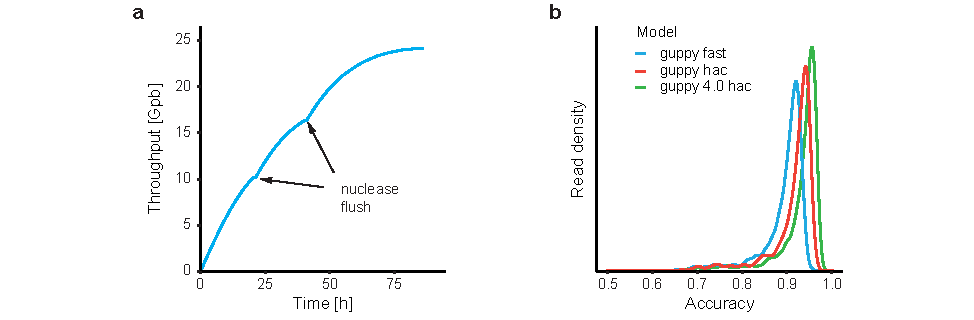
\includegraphics[width=1.0\textwidth]{figures/state_of_art/throughput.pdf}
    \captionsetup{format=plain}
    \caption[Throughput and accuracy]{Throughput and single read accuracy. \textbf{a}, Cumulative sequencing throughput over time of one representative MinION flow cell. Nuclease flushes unblock clogged pores and reload the flow cell with a new library. \textbf{b}, Density plot comparing single read accuracy (BLAST identiy) of 4k random reads basecalled with fast and high-accuracy model of \textit{Guppy} v3.5 and high-accuracy model of \textit{Guppy} v4.0 (Median accuracy: 0.90, 0.93, 0.95; Modal: 0.92, 0.94, 0.95).}
    \label{fig:state_of_art:throughput}
\end{figure}

\begin{figure}[h]
    \centering
    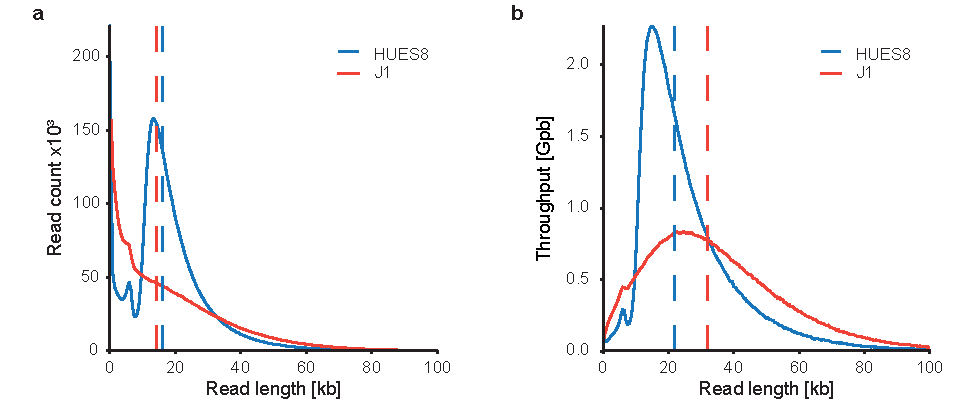
\includegraphics[width=1.0\textwidth]{figures/state_of_art/read_length.pdf}
    \captionsetup{format=plain}
    \caption[Read length median and N50]{Read length distribution: \textbf{a}, Read length distributions shown as number of reads per length (bins of 500nt) of two PromethION flow cells loaded with libraries from different DNA extraction methods. Dashed lines show median read length at 15883 (HUES8) and 14281 (J1). \textbf{b}, Read length distributions shown as sequenced basepairs per read length. Dashed lines show N50 at 21041 (HUES8) and 31906 (J1).}
    \label{fig:state_of_art:read_length}
\end{figure}

\begin{figure}[h]
    \centering
    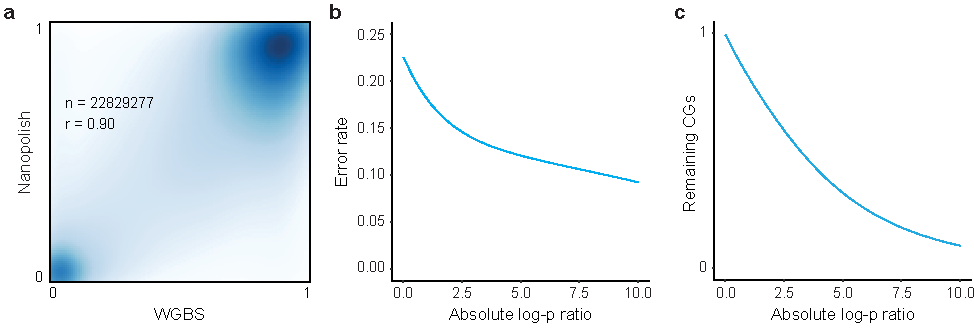
\includegraphics[width=1.0\textwidth]{figures/state_of_art/methylation.pdf}
    \captionsetup{format=plain}
    \caption[Nanopore methylation detection]{Nanopore 5mC methylation detection: \textbf{a}, Correlation of whole genome bisulfite sequencing (WGBS) and nanopore sequenced mean methylation rates per genomic position (\textit{Nanopolish} detection with abs. log-p threshold: 2.5, min. coverage: 10X, reference hg19). \textbf{b}, Detection error depending on the applied absolute log-likelihood ratio (methylation probability) threshold. \textbf{c}, Fraction of dataset remaining depending on log-p value threshold.}
    \label{fig:state_of_art:methylation}
\end{figure}




\section{Summary}
\label{sec:stat_of_art:summary}


Review: Successful test launch for nanopore sequencing \cite{Loman2015a}

Real-time selective sequencing using nanopore technology \cite{Loose2016}







